\documentclass[12pt]{article}
\usepackage[margin=1.2in]{geometry}
\usepackage{comment} 
\usepackage{amsmath}
\usepackage{graphicx}
\title{A report on: Pattern formation by vasculal mesenchymal stem cells}
\date{\vspace{-5ex}}

\begin{document}
	
	\maketitle
	
	\section{Introduction}
	
  In 1952 Alan Turing published his seminar work "The Chemical Basis of Morhogenesis" in which he described the development of complex patterns from originally uniform distributions of chemical substances. This process occurs through the catalytic interaction and simultaneous diffusion of two or more morphogens. The most innovative feature of this model is the introduction of a "reaction" that produces the morphogens. Using only diffusion, local sources of morphogens are needed to form the gradient. Thus the positional information made by the system depends on the prepattern.However by inserting the reaction the system becomes independent. Subsequently the idea has become a critically important foundation to models in many subfields of theoretical biology.
  
  Garfinkel and al. formulate a quantative model of the morphogenesis of vascular mesenchymal stem cells based on reaction-diffusion equations describing the concentration of bone morphogenetic protein 2(BMP-2; a promoter of cell growth, i.e. the activator morphogen) and its inhibitor matrix carboxyglutamic acid protein (MGP). Using numerical methods, they were able to simulate the evolution of their model system under different conditions and recreate a number of experimental observations, thereby applying the explanatory potential of the model to a real physiological mechanism. Crucially, the describe the importance of the ratio between both the diffusivity and the rate of the decay of BMP-2 and MGP for the formation of trabecular patterns. 
  
  Before starting the analysis of the reaction diffusion model of Garfienkel, it is essential to consider the biology that underlies the system. 
  In embryonic development, a mesenchymal stem cell is a progenitor cell which divides over and over and differentiates through a series of transitions into a variety of phenotypes such as cartilage, bones, tendon, ligament, marrow stroma and connective tissues.
  This characteristic migratory, space-filling ability is the keystone of all wound repair in adult organisms, involving mesenchymal cells in the skin (dermis), bone (periosteum), or muscle (perimysium). In diseases like diabetes, atherosclerosis and aortic valvular stenosis, ectopic bone, fat, cartilage and marrow stroma often develop in arteries and cardiac wall. This ectopic tissue shapes focal and nodular patterns in a patchy distribution throughout the vasculature. 
  
  In general pattern formation is the process by which a specialized cell, the fertilized egg, divides to give rise to apparently identical cells. These cells take on different course and become organized into functional organ systems. 
  Within a single organ, such as the heart, multiple classes of differentiated cells must synchronize their duties to ensure that the organ as a whole is functional. 
  One of the unifying principles of development is the idea that embryogenesis proceeds via the iterative process of generating naïve fields of cells, and then providing cells within each field with unique positional information, which they then depict to give rise to spatial patterns.
  
  
  We can model mathematically pattern formation by assuming morphogens that react chemically and diffuse,as mentioned above. Morphogens are signaling molecules that are released from dynamic localized sources and establish a graded distribution to form a concentration gradient. They elicit distinct cellular responses in a manner that governs the pattern of tissue development in the process of morphogenesis or pattern formation. 
  The concentration gradients of morphogens provide individual cells within a field with positional information, which is interpreted to give rise to spatial patterns.
  \section{Model}
  A number of mathematical models were proposed for reaction-diffusion systems, but most of them followed Turing's basic idea.
  Keller-Segel models	for chemotaxis of single-celled organisms form the beginning of pattern formation modeling. Gierer and Meinhardt also proposed the activator-inhibitor model,which can be used to explain the formation of polar, symmetric and periodic structures (spots on animals). Garfinkel et al constructed a simplified model of the vascular mesenchymal cell pattern formation process based on the model of Gierer and Meinhardt.
  \subsection{Model and Parameter selection}
  Alan Garfinkel and his partners treated this model as 2D spatial domain in 100*100 uniform mesh.The activator(BMP-2) and inhibitor (MGP) corresponds to U(x,y) and V(x,y) (effective concentrations). 
  The final concentrations for BMP-2 and MGP were calculated using second order Runge-Kutta time integration scheme.
  Moreover the chemical kinetics they chose were the interactions of BMP-2 with MGP. Additionally, in order to govern the model equations, the initial condition is described as following “The initial condition of U and V that are uniformly distributed with a 2\% random perturbations” as well as neumann conditions (no-flux at boundary) for their boundary conditions. Thus the whole equations are the following: 
  \begin{equation}
  \frac{\partial U}{\partial t}=D({\nabla}^2 U) + \gamma[\frac{U^2}{1+k{U}^2V}] - cU	
  \label{eq:1}
  \end{equation}
  
  \begin{equation}
  \frac{\partial V}{\partial t}=({\nabla}^2 V) + \gamma{U^2} - eV + S
  \label{eq:2}
  \end{equation}
  In these above equations, D is the ratio of diffusion coefficient of BMP-2 and MGP which is $D_u / D_v$ (BMP-2 and MGP respectively). $\gamma$ is the scaling parameter which is equal to $\frac{L^2}{D_v T_C}$, where $L$ is the length of the domain which is the actual size in their experiments, $T_C$ is the time for BMP-2 synthesis. $k$ is the saturating value. $c$ and $e$ are the first order degradation rates for BMP-2 and MGP. $S$ is source term.
  
  More precisely, in equation 1, BMP-2 will activate its own production autocatalytically which will saturate. Hence Garfinkel et al chose $\frac{U^2}{1+k U^2}$, a sigmoidal form, to govern this autocatalysis. V is treated as the inhibitor in the denominator. There is a degradation for U at rate c. In equation 2, $U^2$ is used to represent that BMP-2 spurs MGP in non-linear manner. There is a degradation for V at rate e. S represents the exogenous MGP which is added by purpose.
  
  In order to run the equations smoothly, the parameters were chosen carefully. Firstly, Garfinkel et al took the initial value of $Du$, $1 \times 10^{-8} cm^2/sec$, directly from Entchev et al’s work which was calculated by using GFP labeling and imaging. Then they considered the diffusion of large amount of molecules in nonlinear slowing manner. Due to acid PH, dimerization of BMP-2 and actual tissue culture, the estimated value reduced to $0.15 \times 10^{-8} cm^2/sec$. Because there is no directly calculated value for diffusivity of MGP, they estimated an theoretical approximate value, $30 \times 10^{-8} cm^2/sec$, which was based on empirical formulas. Meanwhile, this approximate value is similar to the diffusion coefficient of amyloid B which is $50 \times 10^{-8} cm^2/sec$. Finally, the value of D was calculated by $\frac{D_u}{D_v} = \frac{1}{200}$.
  
  In the previous experiment which was done by Ghosh-Choudhury et al, it shows that BMP-2 autoregulates in a saturating manner. However, due to unknown level of MGP, it is difficult to establish the precise value of k. In Garfinkel et al’s model, they chose k=0.65.
  
  In order to calculate , it is essential that production rates are known. In previous work, they have found the upper limit for the production rate which is in embryonic kidney cells with a cytomegalovirus (CMV) promoter. They also established the rates for BMP-2 production in calcifying vascular cells and in endothelial cells which were both . Furthermore, FLAG-tagged MGP and newly developed ELISA suggested that the production rates of BMP-2 and MGP are similar. These reports can inform that the upper limit for the production rates is  and the lower limit is .
  
  As mentioned above,  is equal to . In the actual cell culture, the is 4cm,  they chose is 1 ng/hr (). Hence the 
  
  Garfinkel et al estimated the degradation rate of BMP-2 directly and conservatively from the calculation of Entchev et al’s work. Hence they took c = 0.01. MGP has more rapidly degradation than BMP-2 based on their unpublished work. The ratio for  is approximately . Thus they took e = 0.02.
  
  The source term S is to be added in order to make tripling pattern formation which means the source term needs to be three times the initial concentration of MGP. In the model, Garfinkel et al chose the initial value of MGP scaled as 2. Then for the 1000 time steps, the S needs to be 0.06 per time steps, totally 6 which will make tripling pattern formation.
  
  \subsection{Non-dimensionalization and Steady States}
  
  Using the scaling factors $u=\sqrt{k}U$, $v=c\sqrt{k}V$ as well as $\tau = \gamma c t$ and $\vec{\xi}=\sqrt{\gamma c} \vec{x}$ we were able to non-dimensionalize the system as
  $$\frac{\partial u}{\partial \tau} = D\nabla^2 u + \frac{u^2}{(1+u^2)v}-u,\ \ \ \frac{\partial v}{\partial \tau} = \nabla^2 v + G u^2 - E v + Z$$
  where $G=\frac{1}{\sqrt{k}}$, $E=\frac{e}{c}$ and $Z=\sqrt{k}S$.
  
  
  The steady state at $(\bar u_0,\bar v_0)=(0,S/E)$ is apparent and quickly confirmed to stable. We found another stable steady state numerically, which suggests the existence of a third, unstable steady state.
  This notion is corroborated in Garfinkel 2008 which additionally provides analytical forms of the non-trivial steady states. We were able to proof the equivalence of the two systems of equations and the analyses from the later paper can thus be applied to  our model. The stable (+) and unstable (-) steady states (for $G=1$, $k=1$, $E=2$) are
  
  $$(u_\pm,v_\pm)=\Bigg(\frac{\sqrt{\theta}\pm\sqrt{\eta}}{2}, \frac{\theta\pm\sqrt{\theta\eta}}{2-(Z-1)\sqrt{\theta}\pm\theta\sqrt{\eta}}\Bigg)$$
  
  where $\eta = \frac{4}{\sqrt{\theta}+\phi}$, $\theta=\frac{\beta/\rho-\rho-2(Z+1)}{3}$, $\phi = -\theta-2(Z+1)$, $\rho = \sqrt[3]{\alpha/2+\sqrt{\alpha^2/4-\beta^3}}$, $\beta = 1+14Z+Z^2$, $\alpha = 108-72Z(Z+1)+2(Z+1)^3$
  
  \subsection{Stability and Bifurcations}
  
  More interesting than the precise values of the steady states are their stability and how they change with parameter Z. In the last section we noted the existence of two stable and one unstable steady state - a bistable system. This is true for a limited range of Z only, as Garfinkel et al. note.
  
  
 \section{Simulation}
 Computer simulation of continuous mathematical equations need to account for the fact that computers can only represent quanitities with finite accuracy. This is achieved by discretizing time and space into a grid, and applying adequate methods to step between the points in the grid by using current values to estimate values at the next position.
 
 \subsection{Discretization Schemes}
 
 As outlined earlier, we used a Runge-Kutta scheme for temporal discretization and Finite Difference schemes for spatial discretization.
 
 \subsubsection*{Runge Kutta}
 
 The Runge-Kutta methods build upon the idea of Euler's method to numerically approximate solutions for initial value problems. They are formulated as
 
 $$Runge Kutta Here$$
 
 In our simulation we used the second order Runge-Kutta method, RK2, to integrate over the value of time derivatives that we determined using the finite difference method.
 
 \subsubsection*{Finite Difference}
 The finite difference methods for stepping through space are based on the Taylor series expansion of the function:
 
 $$f(x+h) = \sum_{n=0}^\infty \frac{h^n}{n!}f^{(n)}(x)$$
 
 Truncating the series after the n-th element adds an error of order $O(h^{(n)})$ [O-notation] to the approximation and applying the truncation for example after n=2 results in 
 
 $$f(x+h)=f(x)+hf'(x)+O(h^2)$$
 
 Which suggests a discrete-time approximation for the derivative of $f(x)$:
 
 $$f'(x)=\frac{f(x+h)-f(x)}{h}+O(h)$$
 
 Where the term $\Delta_h[f](x)=f(x+h)-f(x)$ is known as the forward-difference. Other variants are central- (a) and backward-difference (b): Other variants are central- (a) and backward-difference (b):
 
 $$\delta_h[f](x)=f(x+\frac{1}{2}h)-f(x-\frac{1}{2}h)$$
 
 $$\nabla_h[f](x) = f(x)-f(x-h)$$
 
 Applying these approximations recursively yields analogous approximations for higher-order derivatives, e.g. the second order derivative using central-difference:
 
 $$f''(x)=\frac{f(x+h)-2f(x)+f(x-h)}{h^2}+O(h^2)$$
 
 
 \subsection{Numerical stability}
 
 A key property of numerical methods is that with decreasing tim-step size they must converge towards the continuous function they are meant to approximate. I.e. the largest deviation of the numerical approximations $x_n$ from its respective exact value $x(t_n)$tends to 0 as time-step size $dt$ goes to 0:
 
 $$\epsilon_N=max_{1\le n\le N}||x_n-x(t_n)||\to0\ \ as\ \ dt\to 0$$
 
 Since the exact values are usually not available - the whole reason for the approximation - we substitute the requirement for convergence with 2 equivalent requirements - consistency and stability. Their equivalence has been proven for finite difference schemes in [Lax 1956] and is thus applicable to our simulation.
 
 Consistency requires that the error $e_n$ introduced at a single time step of the numerical method $\Phi$ tends to 0 as $dt$ goes to 0:
 
 $$e_n = x(t_n+dt) - \Phi(x(t_n),t_n,dt),\ \ \sum_{n=1}^N|e_n|\to 0\ \mathrm{as}\ dt\to 0$$
 
 Since the truncation error $O(\cdot)$ in our simulation is a polynomial in $dt$ this criteria holds.
 
 
 Stability is the requirement that the error due to approximation does not increase faster than linearly with time. 
 
 To determine the stability of a finite difference scheme we can employ the von Neumann stability analysis. The method makes use of a representation of the solution of the PDE as a Fourier series expansion $u_j^k=r^ke^{ij\beta \Delta x}$, where both pairs, the time index $k$ in the LHS and the exponent $k$ of the amplification factor $r$, as well as the spatial index $j$ on both sides of the equation, have the same values, respectively. Substituting the RHS into a finite difference scheme yields, for a 1D linear diffusion equation with central difference:
 
 $$\frac{u_j^{k+1}-u_j^k}{\Delta t} = D\frac{r^ke^{i(j+1)\beta \Delta x}-2r^ke^{ij\beta \Delta x}+r^ke^{i(j-1)\beta \Delta x}}{\Delta x^2}$$
 
 \medskip
 which can be simplified to
 \smallskip
 
 $$r=1+\frac{D \Delta t}{\Delta x^2}(e^{i\beta \Delta x}+e^{-i\beta \Delta x}-2)\ \to\ r=1-4\frac{D \Delta t}{\Delta x^2} \mathrm{sin}^2(\beta\Delta x/2)$$
 \smallskip
 
 yielding $\Delta t < \frac{\Delta x^2}{2D}$ as the condition for stability. Our attempts to apply this analysis to our system of equations failed a) because of the nonlinearities and b) it being a system rather than a simple PDE (i.e. V occurs in the equation for $U_t$).
 
 \subsection{Implementation}
 
 In the paper Garfinkel, et al. inform us that they used a finite difference method with second order Runge Kutta. To allow for comparison between their results and ours, we implemented our simulations in Python using the aforementioned methods.
 
 Utilizing the matrix operations in Numpy we were able to formulate the different schemes as arithmetic operations between the shifted spatial grid.
 
 $$MATRIX FORMULATION?$$
 
 We were able to retrace the simulations and results presented in the article, using an explicit forward time, central difference scheme (FTCS). In the supplements to the article Garfinkel et al. described for the cell density as
 
 $$\frac{\partial N}{\partial t}=\nabla^2N-\frac{\chi_0}{1+U^2}\nabla U \nabla N- \nabla(\frac{\chi_0}{1+U^2}\nabla U)N$$
 
 Despite best efforts, we were not able to simulate the nonlinear PDE. Following the advice of our advisor, Dr. Reuben O'dea, we tried to mitigate the appearing numerical instability using an upwind scheme, but were not able to prevent blow-up in the simulation.
 
 The idea behind the upwind scheme is to deal with the advection term in the PDE by compensating for the acceleration caused by advection in the characteristics between $u^n$ and $u^{n+1}$ in order to assure that the domain of numerical dependence contains the domain of analytical dependence.
 $$GRAPHIC\ for\ METHOD\ OF\ LINES$$
 
 \pagebreak
 
 \section{Results}
 
 We decided to first check some assertions made in the original paper. The authors suggest that the appearance of Turing patterns is critically dependent on the ratio of the morphogens' diffusion constants, $D_u$ having to be smaller than $D_v$. Varying the value of $D_v$ while keeping $D_u$ fixed at 0.01 we observed the disappearance of Turing patterns as $D_v$ approaches and passes that of $D_u$ (Fig. 1).
 
 \begin{figure}[h!]
 	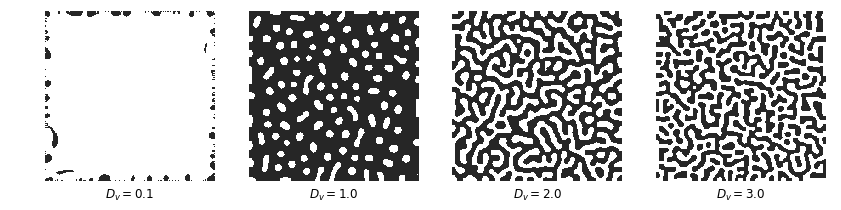
\includegraphics[width=\linewidth]{diffusivity.png}
 	\caption{Figure 1: Varying Diffusivity}
 	\label{fig:dv}
 \end{figure}
 
 Next we tested the assertion that the width of the stripes in the Turing pattern varies with changes in the timescale $\gamma$, where a larger $\gamma$ is expected to result in thinner stripes. The simulations in Fig. 2 confirm this.
 
 \begin{figure}[h!]
 	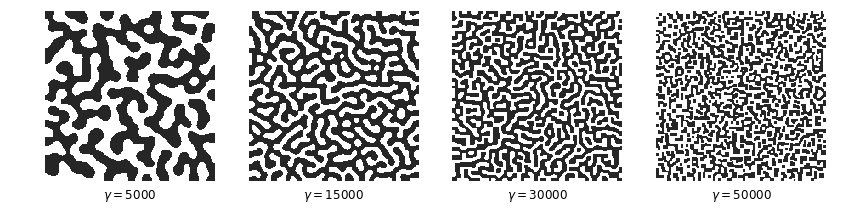
\includegraphics[width=\linewidth]{timescale.png}
 	\caption{Figure 2: Varying Timescale}
 	\label{fig:gamma}
 \end{figure}
 
 Most importantly, Garfinkel et al. describe a qualitative variation in the appearing patterns depending on the magnitude of the external inhibition S. Garfinkel described this in more rigorous terms in []. We were indeed able to confirm the distinct types of patterns across the parameter space. Varying the parameter $S$ from 0 to 0.5 we discovered that the system exhibited largely uniform states with holes and spots at the low and high end of the interval, respectively. In the range between we observed the appearance of a negative pattern that inverted around the value $S=0.125$ to display a positive labyrnth pattern, transitioning through a region (~[0.3,0.4]) displaying fragmented stripes into spots.
 
 \begin{figure}
 	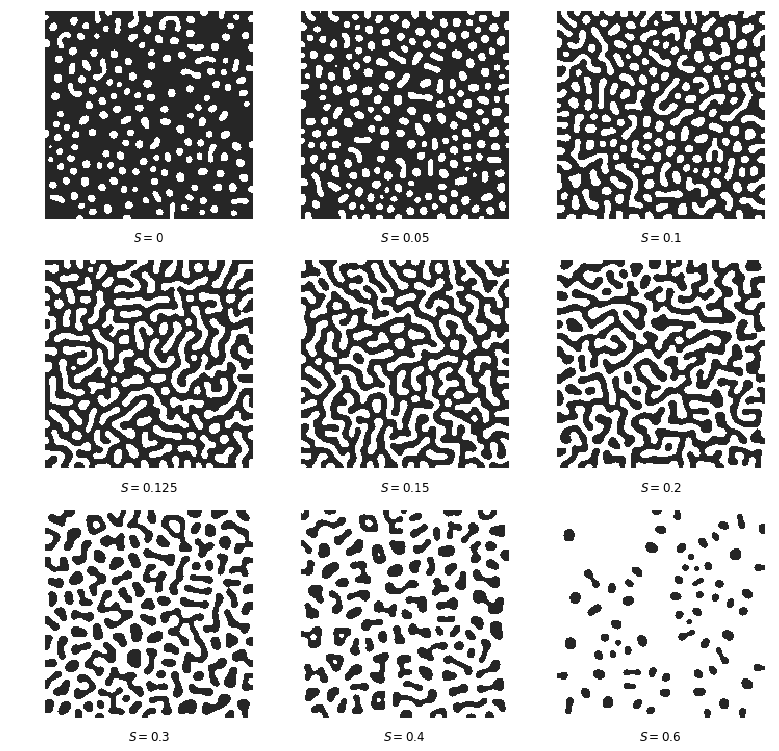
\includegraphics[width=\linewidth]{inhibition.png}
 	\caption{Figure 1: Varying external inhibition}
 	\label{fig:s}
 \end{figure}

\begin{thebibliography}{}
 \bibitem{Mesenchymal Stem Cells}
 Caplan, A. I. (1991). Mesenchymal stem cells. \textit{Journal of orthopaedic research, 9}(5), 641-650.
 
 \bibitem{Morphogen Gradients}
 Christian, J. L. (2012). Morphogen gradients in Development: from form to function. \textit{Wiley Interdisciplinary Reviews: Developmental Biology 1}(1):3-15.
 
 \bibitem{Garfinkel 2004}
 Garfinkel, A., Tintut, Y., Petrasek, D., Boström, K., \& Demer, L. L. (2004). Pattern formation by vascular mesenchymal cells. \textit{Proceedings of the national academy of sciences of the United States of America, 101}(25), 9247-9250.
 
 \bibitem{Garfinkel 2008}
 Yochelis, A., Tintut, Y., Demer, L. L., \& Garfinkel, A. (2008). The formation of labyrinths, spots and stripe patterns in a biochemical approach to cardiovascular calcification. \textit{New Journal of Physics, 10}(5), 055002.
 
 \bibitem{Lax 1956}
 Lax, P. D., \& Richtmyer, R. D. (1956). Survey of the stability of linear finite difference equations. \textit/{Communications on pure and applied mathematics, 9}(2), 267-293.
 
 \bibitem{Turing 1952}
 Turing, A. M. (1952). The chemical basis of morphogenesis. \textit{Philosophical Transactions of the Royal Society of London. Series B, Biological Sciences, 237}(641), 37-72.
 
 \bibitem{Keller Segel 1970}
 Keller, E. F., \& Segel, L. A. (1970). Initiation of slime mold aggregation viewed as an instability. \textit{Journal of Theoretical Biology, 26}(3), 399-415.
 
 \bibitem{Gierer Meinhardt 1972}
 Gierer, A., \& Meinhardt, H. (1972). A theory of biological pattern formation. \textit{Kybernetik, 12}(1), 30-39.
 
 \bibitem{Reaction-Diffution-Turing}
 Shigeru Kondo, et al., (2010).Reaction-Diffusion model as a framework for understanding biological pattern formation,\textit{ Science}, 329, 1616 .
  
 \bibitem{Morphogens}
 Tetsuya Tabata, Yuki Takei, (2004). Morphogens, their identification and regulation
 \textit{ Development 131}, 703-712.  
 
\end{thebibliography}

\end{document}